%
% A3
%
\chapter[Mathematics]{Mathematics for social scientists}%
  %
  %
  \label{ch:math}%
	\index{Mathematics}%
	%
	%




Many aspects of human survival are related to events, objects or people that can be enumerated. For example, infant mortality, forced migration and market collapse are all quantifiable social problems for which we might want to know how frequently they occur, and under what circumstances. A lot of applied mathematics is therefore used in the formalization of markets, populations and disease, both for industrial and for research purposes.

To manipulate things in mathematical form, we rely on symbols and conventions to write down expressions like $y = f(x)$ (the function $f$ that returns the value $y$ for a value of $x$).

%
\paragraph{Greek letters}%
%
Table~\ref{tbl:greek} references the Greek letters that are used in conventional notation: if you read a lot of science-fiction, you might be able to skip this, otherwise start familiarizing yourself with them. In practice, we will use only a subset of the Greek alphabet, and we will use only a few letters at a time.

\begin{table}%

$$
\begin{array}{r*5lrl}
\multicolumn{6}{l}{\text{\textbf{Lowercase}:}} &\multicolumn{2}{l}{\text{\textbf{Uppercase}:}}\\[.5em]
\alpha		& \text{alpha}			& \kappa	& \text{kappa}			& \tau		& \text{tau}		& \Gamma		& \text{Gamma} \\
\beta		& \text{beta}			& \lambda	& \text{lambda}			& \upsilon	& \text{upsilon}	& \Delta		& \text{Delta} \\
\gamma		& \text{gamma}			& \mu		& \text{mu}				& \phi		& \text{phi}		& \Theta		& \text{Theta} \\
\delta		& \text{delta}			& \nu		& \text{nu}				& \varphi	& \text{var-phi}	& \Lambda		& \text{Lambda} \\
\epsilon	& \text{epsilon}  		& \xi		& \text{xi}				& \chi		& \text{chi}		& \Xi			& \text{Xi} \\
\varepsilon	& \text{var-epsilon}	& \pi		& \text{pi}				& \psi		& \text{psi} 		& \Pi			& \text{Pi} \\
\zeta		& \text{zeta}			& \varpi	& \text{var-pi}			& \omega	& \text{omega}		& \Sigma		& \text{Sigma} \\
\eta		& \text{eta}			& \rho		& \text{rho}			&			&					& \Upsilon		& \text{Upsilon} \\
\theta		& \text{theta}			& \varrho	& \text{var-rho}		&			&					& \Phi			& \text{Phi} \\
\vartheta	& \text{var-theta}		& \sigma	& \text{sigma}			&			&					& \Psi			& \text{Psi} \\
\iota		& \text{iota} 			& \varsigma	& \text{var-sigma}		&			&					& \Omega		& \text{Omega}
\end{array}
$$
  
  \caption{Greek letters}\label{tbl:greek}
\end{table}

% You can read sequences of letters and numbers by simple enunciation: $\Delta x$ is pronounced ``delta-x'' and $\beta_1X_1$ is pronounced ``Beta-One X-One''. Note that the pronunciation of Greek letters varies from your linguistic standard: $\chi^2$, for example, designates the ``Chi-squared'' value, which is pronounced ``Kai-squared''.

%
\paragraph{Mathematical symbols}%
%
Table~\ref{tbl:math} references some common math symbols that are used to compose expressions such as: for every ($\forall$) nonnegative real number $(x \in \mathbb{R}^{+})$, there exists ($\exists$) a square root number given by the function $f: x \rightarrow \sqrt{x}$. Again, we will use only a few of these symbols for demonstration purposes.

\begin{table}%

$$
\begin{array}{rlrlrlrl}
\exists  	    & \text{there exists}	            & |x|      	  & \text{absolute value, determinant}			& \Sigma      & \text{summation}              \\
\forall		    & \text{for all/any}	            & [...]       & \text{closed interval}			            & \Pi         &  \text{product}               \\
\therefore		& \text{therefore}	              & (...)       & \text{open interval}    				        & \Delta x    & \text{the change in } x       \\
\Rightarrow		& \text{implies}			            & \{...\}     & \text{set}	                  			    & \partial	  & \text{partial differential}   \\
\to  & \text{goes to, approaches}  	            & \varnothing & \text{empty set}      		              & \int		    & \text{integral}               \\
\mid          & \text{such that, given}     	  & \subseteq   & \text{is a subset of}       			      & x!		      & \text{factorial}              \\
\text{iff}    & \text{if and only if}			      & \subset     & \text{is a proper subset of}			      & \ln(x)	    & \text{natural logarithm}      \\
\in           & \text{is an element of}		      & \cup        &	\text{union}                            & \log_b(x)		& \text{logarithm of base } b   \\
\notin        & \text{is not an element of} 		& \cap		    &	\text{intersection}                     &	x^k   	    & x \text{ at power/exponent } k\\
\approx       & \text{equals approximately}     & \infty      & \text{infinity}                         & \sqrt{x}    & \text{square root of } x      \\
\simeq        & \text{approximately equal to}   & \lim        & \text{limit}                            & \sqrt[3]{x} & \text{cubic root of } x       \\
\end{array}
$$
  
  \caption{Selected mathematical symbols and expressions}\label{tbl:math}
\end{table}


Some letters have standard representations in statistics, such as $\mu$ and $\bar X$ for the population and sample means, $\sigma$ and $s$ for standard deviation, $\sigma^2$ and $s^2$ for variance, etc. You will learn these conventions through practice. Using a computer will introduce slight deviations to these conventions because statistical software like Stata might denote, for instance, $\chi^2$ as \texttt{chi(2)}.

%
\paragraph{Numbers}%
%
Positive numbers like $5, 10, 4$ (the $+$ sign can be omitted) and negative numbers like $-3, -1$ are called integers. If a number $x$ has no floating point (decimals), you are looking at an integer.

The set of \emph{natural} numbers $\mathbb{N}$ contains positive integers $1,2,3,4, \ldots, $ and eventually contains $0$ if you need it to. These numbers can be ordered to form a coordinate system centred around $0$, as shown below:

\begin{figure}[h]
  \begin{tikzpicture}[x=0.75cm,>=stealth]
    \draw[<->] (-5,0)--(5,0);
    \foreach \x in {-4,...,4}
    \draw[shift={(\x,0)},color=black] (0pt,2pt) -- (0pt,-2pt) node[below] {\footnotesize $\x$};
    \node[above,color=s1] at (7.5,15pt)  {irrational numbers};
    \draw[color=s1] (1.41,0) -- (1.41,15pt);
    \node[above,color=s1] at (1.41,15pt) {$\sqrt{2}$};
    \draw[color=s1] (2.71,0) -- (2.71,15pt);
    \node[above,color=s1] at (2.71,15pt) {$e$};
    \node[below,color=s2] at (7.5,-15pt)  {rational numbers};
    \draw[color=s2] (-1/2,0) -- (-1/2,-15pt);
    \node[below,color=s2] at (-1/2,-15pt) {$-\frac{1}{2}$};
    \draw[color=s2] (9/4,0) -- (9/4,-15pt);
    \node[below,color=s2] at (9/4,-15pt) {$\frac{9}{4}$};
    \node[below] at (-5,-5pt)  {$\ldots$};
    \node[below] at (5,-5pt)   {$\ldots$};
  \end{tikzpicture}
  \caption{The real number line.}
\end{figure}

The numbers covered by that coordinate system are said to be rational if they can be expressed as a ratio of two integers $r = \frac{n}{d}$ with $d \neq 0$. Numbers that cannot take the form of a ratio, like $\sqrt{2}$ or the mathematical constant $e$, are said to be irrational.

Numbers belong to sets. The set of \emph{real} numbers $\mathbb{R}$ contains the continuum of all rational and irrational numbers. This set designates a system of coordinates called the real number line, from which you get intervals, Cartesian planes, and the rest of the mathematics that we will use.

%
%
%
\section{Functions}

\newthought{A function} is a rule that describes a relationship between numbers. For each number x, a function assigns a unique number y according to some rule. Thus a function can be indicated by describing the rule, as “take a number and square it,” or “take a number and multiply it by 2,” and so on. We write these particular functions as y = x2, y = 2x. Functions are sometimes referred to as transformations.%

%
%
\subsection{Operators}

%
\paragraph{Summation}%
  %
  When you add all values of $X$ over $n$ observations $X_1, X_2, \ldots, X_n$, you are \emph{aggregating} the values of $X$ over $i = 1, 2, \ldots, n$ observations. Summation notation uses the $\Sigma$ letter to represent this operation:%

  $$\sum_{i=1}^n X_i = X_1 + X_2 + \cdots + X_n$$

  The $X_1 + X_2$ relationship is \emph{additive}, and a subtraction is simply a negative addition: $a-b=a+(-b)$. The identity number for addition and subtraction is 0: if you add or subtract 0 to a value, nothing happens to that value (it stays equal).%

\paragraph{Product}%
  %
  When you multiply all values of $X$ over $n$ observations $X_1, X_2, \ldots, X_n$, you are looking at the \emph{product} of $X$ over $i = 1, 2, \ldots, n$ observations. Product notation uses the $\Pi$ letter to represent this operation:%

  $$\prod_{i=1}^n X_i = X_1 \times X_2 \times \cdots \times X_n$$

  The $X_1 \times X_2$ relationship is \emph{multiplicative}, and a division is simply an inverse multiplication: $\frac{a}{b} = a \cdot \frac{1}{b}$. Their identity number is 1: if you multiply or divide a value by 1, nothing happens to that value.%

  % If the world were organized as in the movie \emph{Highlander}, the ultimate issue is the survival of one, hence the memorable tagline of the movie: ``There can be only one''. The limit of the \emph{Highlander} universe is 1 because every fight between two Immortals systematically leads to one less living Immortal. The limit of $x/2$ for $x > 1$ is 1.

%
%
\subsection{Exponentials}

Power functions feature an exponent $k$ to raise $x$ to a given power, such that $f(x) = x^k = x*x*...*x$ ($k$ times). Some examples of power functions, where the exponent is constant, are shown in Figure~\ref{fig:exps-and-powers}.%

%
\paragraph{Example: Scientific notation}%
%
Power functions are useful to rewrite large numbers with the function $f: x \to a \times 10^b$, where $a$ is any real number and $b$ is an integer. For example, by the end of August 2012, the U.S. national debt amounted to \$\href{http://www.treasurydirect.gov/NP/BPDLogin?application=np}{16,015,769,788,215.80}. This number can also be written as $16 \times 10^{12}$, \ie 16 trillion, or as \ensuremath{1.6\times 10^{13}} in scientific notation.

%
\paragraph{Exponentials}

Exponential functions are also useful to handle some phenomena like the exponential growth of the population or labour force in many countries, or the exponential decay of an organism or technology.

\begin{knitrout}
\definecolor{shadecolor}{rgb}{0.969, 0.969, 0.969}\color{fgcolor}\begin{figure}[]

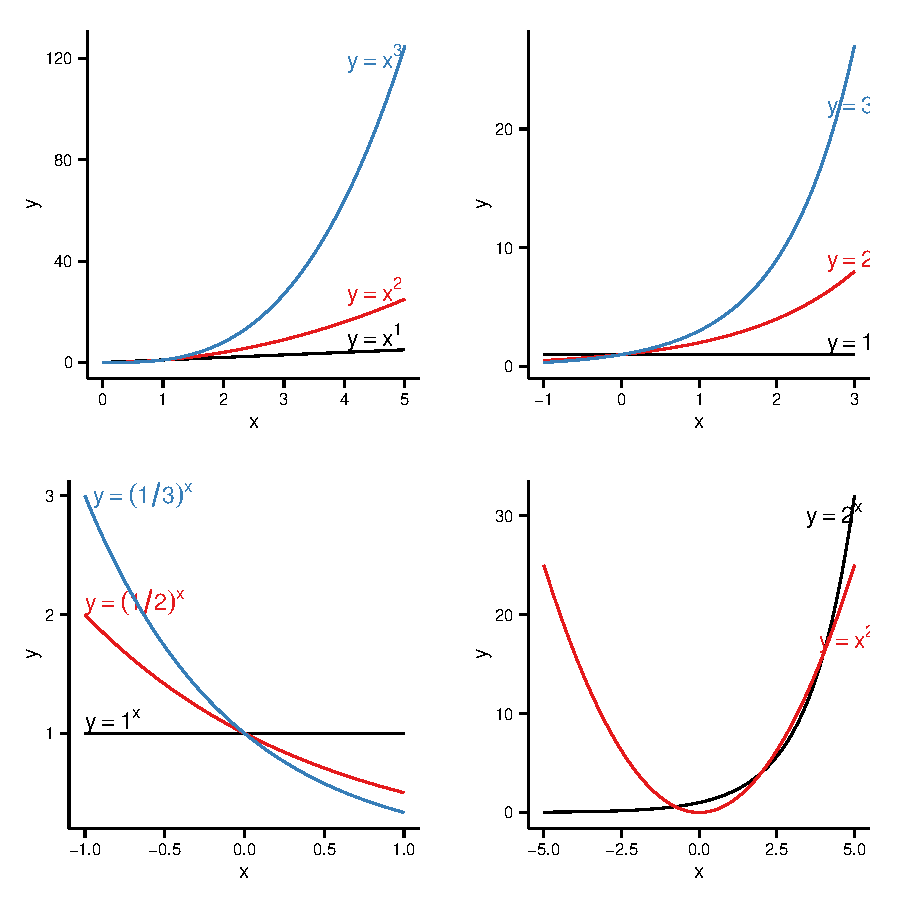
\includegraphics[width=\linewidth]{images/math-exps-and-powers} \caption{Top-left: visualization of the power functions $y = x^k$ for $k = [1,2,3]$. In the case where $k = 1$, the growth of $y$ is linear because $y = x$. All three curves are examples of strict monotonicity, \ie a systematic increase of $y$ when $x$ increases. Top-right: exponential functions. Bottom-left: positive fractional exponentials (decay functions). Bottom-right: comparison of power and exponential progression near $0$.\label{fig:exps-and-powers}}
\end{figure}


\end{knitrout}


%
%
\subsection{Logarithms}

Logarithms are a way to reverse the transformation of an exponential function: $y = log_b x \iff b^y = x$. The logarithm can take any base $b > 0$.

%
\paragraph{Example: $y = \log_2(x)$} %
%
Early game consoles were often advertised through their bit ratings, which progressed exponentially from 8-bit to 64-bit processors. The geometric progression of their corresponding exponential function, $y = 2^x$, can also be described as the linear progression of its logarithm of base 2:

\begin{itemize}
  \item $y(3) = 2^3 = 8$ \quad then, by definition: \quad $\log_2(8) = 3$
  \item $y(4) = 2^4 = 16$ \quad then, by definition: \quad $\log_2(16) = 4$
  \item $y(5) = 2^5 = 32$ \quad then, by definition: \quad $\log_2(32) = 5$
  \item $y(6) = 2^6 = 64$ \quad then, by definition: \quad $\log_2(64) = 6$
\end{itemize}

%
\paragraph{Natural logarithm}

The natural logarithm of base $e$ is denoted $\ln(x)$ or simply $\log(x)$, such that $\ln(x)=e^x$.

\begin{knitrout}
\definecolor{shadecolor}{rgb}{0.969, 0.969, 0.969}\color{fgcolor}\begin{figure}[]

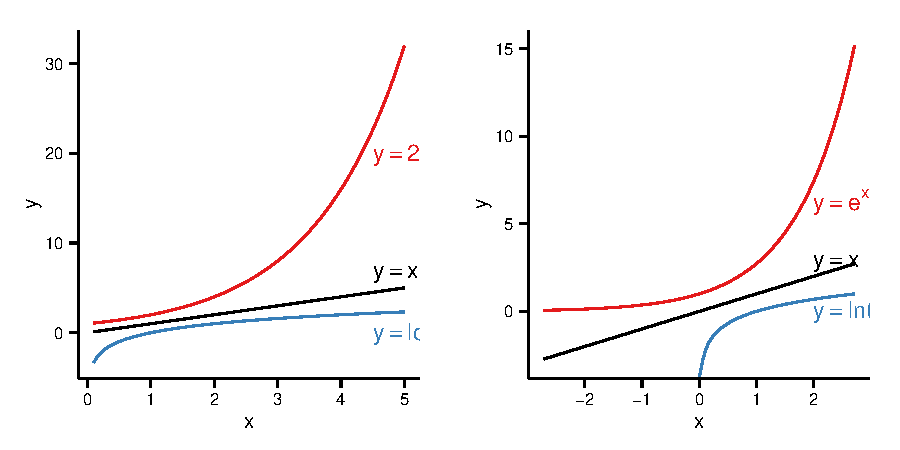
\includegraphics[width=\linewidth]{images/math-exps-and-logs} \caption{Left: logarithmic vs. exponential functions. Right: natural logarithm vs. exponential functions.\label{fig:exps-and-logs}}
\end{figure}


\end{knitrout}


Hi.

% Another application is the (heavily subsidised) production of ethanol in the United States, which has grown quasi-exponentially during the 20th century.
% http://www.graphoftheweek.org/2012/02/massive-increase-in-ethanol-production.html
% http://www.graphoftheweek.org/2012/06/body-weight-in-united-states-part-3.html

\section{Derivatives}
  \subsection{Rates of change}
	\index{Descriptive statistics!Growth rates}%
	\index{Growth rates}%
%
The proportion of change in a measurement over time is referred to as its \textbf{growth rate}:

\begin{itemize}
	\item If your measurement is itself an average value, the growth rate of a mean $\bar{X}$ at time $t$ is calculated as $g = \frac{\bar{X}_t - \bar{X}_{t-1}}{\bar{X}_{t-1}}$, or $100 \cdot g$ if you want to express the growth rate as a \textbf{percentage change}.

	\item If the variable $X$ represents a proportion, do not confuse the growth rate and its percentage change with the change in \textbf{percentage points}. For example, if a political party doubles its electoral support and goes from 15\% to 30\% of the vote share, its progression of 15 percentage points translates into a $100 \cdot \frac{.3-.15}{.15} = 100\%$ growth.
	
	\item Under some circumstances, you might prefer to use a \textbf{fixed index} value $\bar{X}_{t0} = 100$ instead of $X_{t-1}$ as the reference value for a rate. The index values of $X$, which you get by calculating $I_X = \frac{\bar{X}_t}{X_{t0}}$, are insensitive to the scale of $X$.
	\end{itemize}

We will come back to growth rates when we learn to use logarithmic transformation, because the trend of $log(X)$ approximates its overall growth rate and the first difference of $log(X)$ approximates the percentage change between $X_{t-1}$ and $X_t$ when the changes are of small amplitude.

% --// ref.
% http://www.duke.edu/~rnau/411log.htm

  
  \subsection{Relative growth rates}

\section{Probability}

  \subsection{Random variables}

  \subsection{Probability distributions}

\section{Statistics}

\subsection{Variables}%
%
Most of our notation uses Roman letters to designate things like variables or values (observations) of these variables. Most commonly, we use $X$ or $Y$ to designate a variable and $n$ to designate its total number of observations. The number of observations will be treated as a sequence that goes from 1 to $n$, and the rank of an observation in that sequence will be noted $i$, with $i = (1,2, \ldots, n)$.%

In this notation, $X_i$ is the value of variable $X$ for observation $i$. The rank $i$ of an observation is meaningless if the units of observations of your sample are randomly selected, but you need the $X_i$ notation to designate the full array of $i = 1,2, \ldots, n$ values taken by the variable $X$ in your sample. %

The rank of an observations can also be turned into a unique identifier for each of your observations, which is useful when you need to program a command of the form:%

\begin{quote}
	\emph{for each} (observation), \emph{do} (this)
\end{quote}

What will generally happen in this scenario is that you will call a function (or write one) that spells out like this:

\begin{quote}
	\emph{for each} $i = (1,2, \ldots, n)$ of $X$, \emph{do} (this) to $X_i$
\end{quote}

This notation is very close to the one used in statistical software, which automatically operates on arrays (rows and columns, making up vectors and matrices) of values.%

\paragraph{Dependence} %
  %
  Often we want to indicate that some variable $y$ depends on some other variable $x$, but we don’t know the specific algebraic relationship between the two variables. In this case we write $y = f(x)$, which should be interpreted as saying that the variable $y$ depends on $x$ according to the rule $f$. Given a function $y = f(x)$, the values of $x$ are often called the \emph{independent} variable, and the values of $y$ are often called the \emph{dependent} variable.%

  `Controls'.

\paragraph{Estimates}%
  %
  As soon as we will start to work with samples of data, we will be handling estimates of values that exist in a larger population. While our \emph{sample} population contains $i = 1,2, \ldots, n$ observations, the \emph{true} population contains $N$ observations, which might be unknown.%

  We will distinguish sample from population parameters with different notations: in a sample, the mean value of $X$ is noted $\bar{X}$, but its true mean value in the actual population is noted $\mu$. We will treat $\bar{X}$ as an estimated value of $\mu$.%

  Estimates are often designated with a hat, as in $\hat{Y}$, which is pronounced ``y~hat''. For example, if your sample contains 25\% of uninsured respondents, the proportion $\hat{p} = .25$ is an estimate of the true proportion of uninsured individuals in your population.%

\subsection{Means}%

Mean values provide the average level of a parameter. They can be calculated in several ways, but \textbf{arithmetic means} are by far the most common. The arithmetic mean of variable $X$ with $n$ observations is written $\bar X$ and pronounced ``x bar''. Its value is given by the following formula:

$$\bar{X} = \frac{X_1 + X_2 + \cdots + X_n}{n} = \frac{1}{n}\sum_{i=1}^n X_i$$

Arithmetic means are computationally simple: they simply aggregate values of $X$ and divide their sum by the overall number of observations $n$. The drawback of this method is that it is not robust to the extreme values of a distribution: very high or very low values might heavily distort an average value.

Mathematically, a solution to the issue of high variability can take the form of a different formula, the \textbf{geometric mean}, which uses the \emph{product} of the values of $X$ and elevates it to the inverse power of $n$. The result is the $n$-th root of $X$:

$$\bar{X}_{geom}=\bigg(\prod_{i=1}^n X_i \bigg)^{\frac{1}{n}} = \sqrt[n]{X_1 \cdot X_2 \cdots X_n}$$

Geometric means are a far better choice of averaging for distributions that follow ``power laws'', but these distributions are rare and easily confused with log-log distributions.

% a = c(10, 2, 19, 24, 6, 23, 47, 24, 54, 77)
% n = length(a) #now n is equal to the number of elements in a
% prod(a)^(1/n) #compute the geometric mean

% http://www.stat.cmu.edu/~cshalizi/2010-10-18-Meetup.pdf

%% Harmonic mean:

% $$H = \frac{n}{\frac{1}{x_1} + \frac{1}{x_2} + \cdots + \frac{1}{x_n}} = \frac{n}{\sum_{i=1}^n \frac{1}{x_i}}, \qquad x_i > 0 \text{ for all } i.$$

% a = c(10, 2, 19, 24, 6, 23, 47, 24, 54, 77)
% 1/mean(1/a) #compute the harmonic mean

\paragraph{Sample means}

% http://lingpipe-blog.com/2012/05/29/averages-vs-means/

If your observations are drawn out of a larger population of units, then your dataset contains a sample and every parameter in the sample is an estimate of its true population value. If your data are randomly sampled, then the mean parameters of your data follow a probability mass function for discrete drawings over the natural numbers $\mathbb{N}$:

$$\mathbb{E}[X] = \sum_{x \in \mathbb{N}} \, x \times p(x)$$

This reads as: the true mean $\mu$ is the sum of all possible sample averages multiplied by their probability of occurrence through a random sampling of observations $x$ over $\mathbb{N} = 1,2,3,4,\ldots$. It works only if the samples are random, or `i.i.d.' (independent and identically distributed).

If you are looking a continuous probability, then the probability density function is calculated over all real numbers $\mathbb{R}$ and is defined as follows:

$$\mathbb{E}[X] = \mu = \int_{\mathbb{R}} \, x \times p(x) \, dx$$



\paragraph{Weighted means}

% If $X_1, X_2, \ldots, X_n$ are weighted by a series of coefficients $w_i$, the weighted arithmetic mean $\bar{X}'$ is given by a different formula, depending on how your weights were designed.
% 
% In the first formula, the coefficients $w_1, w_2, \ldots, w_n$ sum up to 1. This notation assigns the influence of $X_i$ on $\bar{X}'$ to $w_i$, which is required if you are averaging over values that correspond to unequal proportions of an overall population.
% 
% $$\bar{X}' = \frac{X_1 w_1 + X_2 w_2 + \cdots + X_n w_n}{n} = \sum_{i=1}^N X_i \cdot \red{w_i}, \qquad \text{with} 0 < w_i < 1 \text{and} \sum_{i=1}^N w_i = 1$$
% 
% Weights are used in surveys where not all individuals have the same likelihood of being sampled.

%% --// CONSUMER PRICE INDEX

% consumer price index: base year, basket of goods, index each price, weight the average of the indices for each year by the budget proportion

%% --// SURVEY WEIGHTS

% http://www.stata.com/help.cgi?weights
% http://www.cpc.unc.edu/research/tools/data_analysis/statatutorial/sample_surveys/weight_syntax

In the second formula, the coefficients $w_i$ do not sum up to 1. Instead, they are directly equal to the influence of the value:

$$\bar{X}' = \frac{X_1 w_1 + X_2 w_2 + \cdots + X_n w_n}{n} = \sum_{i=1}^N X_i \cdot \hlred{w_i}, \qquad \text{with} \sum_{i=1}^N w_i = 1$$

% cancer rates: crude, per pop, weighted EU-15, weighted EU-27, standardised

Using country-level real GDP/capita, measured by the \href{http://unstats.un.org/unsd/snaama/}{United Nations Statistics Divisions -- National Accounts} in 2009:

$$\textsf{Real GDP/capita} = \frac{\textsf{Real GDP}}{\textsf{population}} = \frac{\text{GDP}}{\text{population}} \cdot \text{price index}$$

\begin{itemize}
	\item The mean can summarise the distribution of real GDP/capita in the full sample ($N = 192$) and/or in each geographical region.
	
	\item Average real GDP/capita will be sensitive to exceptionally high or low values, as with Somalia, Liechtenstein or Switzerland.
			
	\item Population and price act like country-level weights: all values of GDP are weighted by $\frac{\text{price index}}{\text{population}}$ to make them comparable.
\end{itemize}

